\documentclass[11pt]{article}

\usepackage[margin=1in,footskip=0.25in]{geometry}

%\usepackage{helvet}
%\renewcommand{\familydefault}{\sfdefault}

\renewcommand\refname{\vskip -1cm}

%\renewcommand{\rmdefault}{phv} % Arial
%\renewcommand{\sfdefault}{phv} % Arial
\usepackage{setspace}
\usepackage{wrapfig}
\usepackage{amsmath}
\usepackage{amssymb}
\usepackage{graphicx}
\usepackage{mathrsfs}
\usepackage{bm}
\usepackage{wasysym}
\usepackage{placeins}
\usepackage{multirow}
\usepackage[T1]{fontenc}
\usepackage[super]{natbib}
\usepackage{framed}
\usepackage{caption}
\usepackage{longtable}

\begin{document}

\title{Isotopic incorporation and the temporal dynamics of foraging among individuals and within populations}
\author{JD Yeakel, U Bhatt, SD Newsome}
\maketitle

\section{Introduction}

Consumer foraging behaviors are dynamic, resulting in diets that change over time as a function of environmental conditions, the densities of consumer and resource populations, and even the physiological states of individual foragers.
Understanding how diets change, and to what extent different conditions promote or inhibit specific changes, is both a challenging theoretical and empirical problem in ecology.

Analysis of carbon and nitrogen stable isotopes of a consumer with respect to a suite of potential prey is a commonly used tool for determining diet.
As a consumer incorporates the isotopic values of its consumed resources into its tissues, it becomes a unique `blend' of its prey.
Determining the most likely proportional contribution of prey that determines a given consumer's diet has thus been the focus of intense interest (REFS).

Of additional interest are the factors that control the consumer's isotopic niche width, which is defined by the isotopic variance of the consumer at either the individual or population level.
A consumer's isotopic niche width, by definition, is a function of the isotopic values of its potential prey (the prey mixing space), as well as its dietary predilections.
For a given mixing space, a consumer with a large isotopic niche width may be incorporating many isotopically distinct prey into its diet, while a consumer with a small isotopic niche width may be specializing on a single resource.


%Difference between the isotopic diet view vs. other diet views

%Backward integrating vs. Forward integrating

%EXPLORE VARIANCE ~ what controls the isotopic niche?

%Prey-switching dynamic
%Micro time frame
%Macro time frame




\section{Methods \& Analysis}
We begin by establishing a forward-integration approach for modeling the incorporation of stable isotopes from multiple resources into the tissue of a consumer.
This new methodology provides an analytical link between the mechanistic drivers of foraging and the distribution of stable isotope values that describe a consumer's tissues over time.
%This framework aims to provide a flexible platform for introducing additional ecological complexities, such as time-dependent foraging behaviors and dietary specialization both among and within individuals.
Using this framework, we aim to
1) examine how certain dietary tendencies, such as prey specialization and different modes of dietary variation, impact the isotopic variance of consumer tissues thus impacting interpretation of the `isotopic niche`, and
2) show how these methods can be expanded to include trophic interactions that themselves are temporally dynamic.

\subsection{Consumer niche width for temporally static diets}
The carbon and nitrogen isotopic composition of a consumer's tissues are a product of its diet.
If this diet incorporates multiple prey in different quantities, as is the case for most consumers, the resulting consumer isotopic distribution must take into account:
\emph{i}) the initial isotopic signature of the consumer's tissues at a point in time $X_c(t)$ (we will assume for simplicity that the isotopic value in question is the ratio of heavy to light carbon isotope relative to a known standard $\delta^{13}{\rm C}$, though are methods are equivalent for any isotope that is integrated through diet),
\emph{ii}) the isotopic values of $n$ resources, which we assume are Gaussian distributed with expectation $\mu_i$ and variance $\sigma_i^2$,
%$\sum_{i=1}^n p_i \mu_i$ (where $p_i$ is the proportional contribution of resource $i$ and $\mu_i$ is the mean isotopic value of resource $i$),
\emph{iii}) the rate at which each prey species is ingested by the consumer, summarized by its proportional contribution $p_i$,
and
\emph{iv}) the incorporation rate of a consumer's diet into its tissue $\lambda$.
In a completely deterministic framework, the isotopic composition of the consumer can be written as an ordinary differential equation

\begin{equation}
\label{eqODE}
\dot X_c = (1-\lambda)X_c + \lambda \sum_{i=1}^N p_i \bar{X}_i - X_c
\end{equation}

\noindent where the overdot denotes the derivative with respect to time $t$.

However, we must also take into account stochastic effects, and here we consider two indepedent sources of variation.
First, each potential resource $i$ has individuals with isotopic values varying according to independent Gaussian distributions with expecation ${\rm E}\{X_i\}=\mu_i$, and variance ${\rm Var}\{X_i\}=\sigma^2_i$.
Secondly, although in this section we consider a consumer diet that does not change over long periods of time, there is variation in the consumption of prey across short periods of time.
In other words, a consumer's diet is described by a probability distribution that itself is temporally static (a constraint that we will ease later on).

%Derivation of the Dirichlet controlling diet
{\bf Deriving the isotopic niche width.} Here we assume that the proportional contribution of prey to a consumer's diet scales to the rate at which it encounters its prey.
%, such that we must first describe how the Dirichlet distribution describing consumer diet at a given point in time changes as a function of prey densities.
A consumer encounters each prey at a frequency determined by a Poisson Process with parameter $\lambda_i$, which determines the number of encounters $N_i(t)=n$ between time 0 and time $t$,

\begin{equation}
f_\Lambda (n_i|\lambda_i) = {\rm e}^{-\lambda_i t}\frac{(\lambda_i t)^n}{n!}.
\end{equation}

\noindent Here and henceforth, we use uppercase notation to denote stochastic variables, and lowercase notation to denote specific values of stochastic variables.
If we assume that encounter rates are variable, such that some prey are more patchily distributed than others, we can treat $\Lambda_i = \lambda_i$ as a random variable with a Gamma density

\begin{equation}
f_\gamma (\lambda_i | c, a_i) = \frac{c^{a_i}}{\Gamma (a_i)}{\rm e}^{-c \lambda_i}\lambda_i^{a_i - 1}.
\end{equation}

\noindent Integrating over all possible values of $\lambda_i$ gives us the Negative Binomial density with mean encounter rate $a_i/c$ and coefficient of variation $1/\sqrt{a_i}$ (REF Mangel).
Following the derivation described by Ainsworth (REF), if we define the proportional contribution of prey to a consumer's diet as

\begin{equation}
  p_i = \frac{\lambda_i}{\sum_{j=1}^n \lambda_j},
\end{equation}

\noindent then $P_i = p_i$ has a Dirichlet distribution with density

\begin{equation}
  f_{\rm Dir}(p_1,...,p_n|a_1,...,a_n) = \frac{\Gamma(\sum_{i=1}^n a_i)}{\sum_{i=1}^n\Gamma(a_i)}\prod_{i=1}^n p_i^{a_i - 1},
\end{equation}

\noindent where $\Gamma(\cdot)$ is the gamma function.
As such, the expected proportional contribution of a prey $i$ to the consumer's diet has an expected value ${\rm E}\{p_i\}=a_i/a_0$ where $a_0 = \sum_i a_i$, and variance

\begin{equation}
  {\rm Var}\{p_i\} = \frac{a_i(a_0 - a_i)}{a_0^2(a_0 + 1)}.
\end{equation}

Describing the dietary behavior of a consumer as a Dirichlet distribution provides a flexible and powerful framework to investigate how different foraging strategies influence a consumer's isotopic niche.
For example, a pure generalist consumer would have a Dirchlet distribution with parameters $a_1 = a_2 = ... = a_n = 1$, such that the marginal distribution for $P_i = p_i$ is close to uniform, such that the expectation is ${\rm E}\{p_i\} = 1/n$.
Because we have assumed that the proportional contribution of a prey to the consumer's diet scales with the prey's encounter rate, this would be analogous to a system where a consumer is equally likely to encounter the same number of any prey.
In contrast, a pure specialist would have a Dirichlet density that is spiked for a given prey $k$, such that the single parameter $a_k \gg 1$, while $a_{i \neq k} = 1$.

%Describing Z
If the isotopic distributions for the set of potential prey follow independent Gaussian distributions, and the dietary behavior of the consumer has a Dirichlet density, the resultant density that describes the isotopic distribution of a consumer's diet $f_Z(Z=z)$ is a weighted mixed Gaussian, with weights determined by $p_{i=1,...n} \sim {\rm Dirichlet}(p_1,...,p_n|a_1,...,a_n)$.
This density can be written as

\begin{equation}
f_Z(Z) = \sum_{i=1}^n \frac{a_i}{a_0}\frac{1}{\sqrt{2 \pi \sigma_i^2}}{\rm e}^{-\frac{(z-\mu_i)^2}{2\sigma_i^2}}
\end{equation}



he expectation for the isotopic distribution of the consumer's diet is

\begin{equation}
\label{eqEZ}
  {\rm E}\{Z\} = \sum_{i=1}^n p_i \mu_i,
\end{equation}

\noindent where $p_i = a_i/a_0$, and $\mu_i$ is the mean isotopic value for prey $i$, and is thus the weighted average of the isotopic values for the prey community.

Of more interest to us here is the variance of $f_Z(z)$, which will allow us to analytically determine the isotopic niche width of the consumer as a function of its dietary behavior and the isotopic distribution of its prey.
We find that

\begin{equation}
\label{eqVarZ}
  {\rm Var}\{Z\} = \sum_{i=1}^n \frac{a_i}{a_0}\left(\sigma_i^2 + \mu_i^2\right) - \frac{a_i^2\mu_i^2}{a_0^2}-\sum_{i \neq j}\frac{a_i a_j \mu_i \mu_j}{a_0^2}.
\end{equation}

\noindent Although the form of Eq. \ref{eqVarZ} is not intuitive, we emphasize that - over different dietary behaviors that shape the Dirichlet distribution and for different isotopic mixing spaces - it is this equation that governs the expansion or contraction of the consumer's isotopic niche width, and therefore of ecological interest.

The isotopic variance of the consumer's diet ${\rm Var}\{Z\}$ can be simplified by considering a specific set of dietary behaviors.
Here we examine how ${\rm Var}\{Z\}$ is influenced by generalist vs. specialist consumer diets, as well as the role of general mixing space geometries.
If a generalist consumer alters its diet to become a specialist on a single prey, the Dirichlet distribution that determines its prey consumption changes from $a_i=1$ for all $i=1,...,n$ to $a_{i \neq k}=1$ for $i=1,...,n$.
As specialization increases, the Dirichlet parameter corresponding to the preferred prey $k$, $a_k$ increases to a value much higher than one (pure specialization is obtained only at the limit $a_k \to \infty$).
Thus, we can assume that $a_i=1$ for all $i \neq k$, and $a_k = (n-1)s/(1-s)$, where $s$ denotes specialization, ranging from 1/n (generalization) to 1 (specialization).
Accordingly, $a_0 = (n-1)/(1-s)$ and $p_i = a_i/a_0 = (1-s)/(n-1)$ for all $i \neq k$, while $a_k/a_0 = s$.
With these substitutions, we find

\begin{equation}
\label{eqVarZs}
{\rm Var}\{Z\} = \frac{1-s}{n-1}\sum_{i \neq k}^n \left(\sigma_i^2 + \mu_i^2\right) + s(\sigma_k^2 + \mu_k^2) - \left(\frac{1-s}{n-1}\sum_{i \neq k}^n \mu_i + s\mu_k \right)^2,
\end{equation}

\noindent and note that, independent of the prey mixing space (a function of $\mu_i$ and $\sigma_i^2$ for prey $i=1,...,n$), the isotopic variance of the consumer's diet will always be a concave parabolic function over $s$.
With respect to the size of the consumer's isotopic niche width, this means that there can be a peak variance for a value of $s$ intermediate to pure generalization ($s=1/n$) and pure specialization ($s=1$).

The peak, or inflection point, that describes the maximum isotopic variance of the consumer may or may not fall between $s=1/n$ and $s=1$, and is only of ecological interest if it does.
This point can be solved exactly by setting the derivative of Eq. \ref{eqVarZs} with respect to $s$ equal to zero, and solving for $s$, such that the inflection point is

\begin{equation}
	\hat s = \frac{A(1-n)+B (n-1)^2+2 C (C-D n+D)}{2 (C-D n+D)^2},
\end{equation}

\noindent where $k$ denotes the prey targeted by the consumer, and $A = \sum_{i \neq k}^n \left(\sigma_i^2 + \mu_i^2\right)$, $B = \left(\sigma_k^2 + \mu_k^2\right)$, $C = \sum_{i \neq k}^n \mu_i$, $D = \mu_k$.


%Integration over time with a static diet
{\bf The Dynamics of Incorporation.}
The isotopic signature of a consumer changes with the consumption of different prey.
The extent of this change is a function of
\emph{i} the difference between the isotopic value of the consumer compared to the isotopic value of its diet, and
\emph{ii} the rate that the isotopic signature of ingested material is incorporated into the consumer, which is tissue-specific $\lambda$.
Because the consumer's diet is stochastic, we must take into account both the isotopic expectation of diet, as well as the isotopic variance of diet, and this will allow us to determine both the expectation and variance of the consumer's isotopic value as a give dietary isotopic distribution is incorporated over time.

The isotopic expectation and variance of the consumer's diet alter the consumer's isotopic signature by the stochastic differential equation

\begin{equation}
\label{eqSDE}
{\rm d}X_c = (1-\lambda)X_c{\rm dt} + \lambda\left({\rm E}\{Z\}{\rm dt} + \sqrt{{\rm Var}\{Z\}}{\rm dW}\right) - X_c{\rm dt}.
\end{equation}

\noindent where ${\rm dW}$ is the increment of Brownian motion.
Because the time interval is extremely short at the continuous time limit, the time evolution of the consumer tissue's isotopic value will be Gaussian distributed, the dynamics of which are formally known as an Ornstein Uhlenbeck process (REF).
In this case, if the initial isotopic values of the consumer is $X_c(0)$, the expectation and variability of $X_c$ at time $t$ are

\begin{align}
{\rm E}\{X_c(t)\} &= {\rm E}\{Z\} + (X_c(0) - {\rm E}\{Z\}){\rm e}^{-\lambda t}, \nonumber \\
{\rm Var}\{X_c(t)\} &= \frac{\lambda {\rm Var}\{Z\}}{2}\left(1 - {\rm e}^{-2\lambda t}\right).
\end{align}

\noindent where ${\rm E}\{Z\}$ and ${\rm Var}\{Z\}$ are as defined in Eqns. \ref{eqEZ} and \ref{eqVarZ}.
This is in accordance with known exponentially-decaying isotopic values of consumers shown in controlled-diet experiments (REFS), as well as a similar derivation in (REF).

%By uniting both dietary and isotopic variability into the single random variable $Z$, the above framework provides a means towards predicting the isotopic composition of a consumer over time, given a dietary strategy (described by the Dirichlet distribution) and the isotopic distribution of the potential resources (the isotopic mixing space).
%Permitting the consumer's dietary strategy to vary provides a direct means of incorporating behavioral variability in estimates of a consumer's isotopic composition.




\section{Results}

%Static results (primary)

%Single prey specialists: If preferred prey has high isotopic variability, the isotopic niche width of the consumer increases with increasing specialization; the generalist niche width is relatively small

%Single prey specialists: If preferred prey has low isotopic variability, both 100% generalism and 100% specialism can have the same isotopic niche width. The intermediate case actually results in a smaller niche width. This is due to (??)
  %The 0,1 values are not interesting... the intermediate specialist values are:
  %The value at '0' is defined by the mean SD of the niche space
  %The value at '1' is defined by the mean SD of the specialized prey
  %The trough at 0.5 is because (I think) of the negative correlations within the Dirichlet distribution... it's due to foraging tradeoffs.


%Multiple prey specialist: When isotopic ratios are sourcing from a small subset of prey, moderate specialization results in smaller niche widths than generalization, and can strongly limit the size of the niche width in general.





\section{Discussion}

\subsection{Static dietary dynamics}



\subsection{Temporal dietary dynamics}
An implicit assumption of the static model is that the consumer's diet varies instantaneously over a given parameterization of $f_Z(Z)$.
This will be relevant for organisms that have a consistently varying diet over time, however most organisms have diets that undergo large shifts over time, such that the Dirichlet distribution that might characterize their diets during one temporal window might be different the the Dirichlet distribution that characterizes their diet in another window in time.
Such a shift might be due to seasonal, ontogenetic, or demographic changes in the consumer's prey base.
In the following section, we will relax the assumption that diet is characterized by a single Dirichlet distribution over time, thus generalizing the dietary/isotopic dynamics as a function of time.

We now assume that diet (but not the isotopic distribution of prey) changes over time, such that the random variable of interest is now $Z(t)$.
Solving for $X(t)$, we find

\begin{align}
{\rm E}\{X(t)\} = X(0){\rm e}^{-\lambda t} + \lambda{\rm e}^{-\lambda t} \int_{s=0}^t {\rm e}^{\lambda s} {\rm E}\{Z(s)\}{\rm d}s, \nonumber \\
{\rm Var}\{X(t)\} = \lambda^2 {\rm e}^{-2\lambda t} \int_{s=0}^t {\rm e}^{2\lambda s} {\rm Var}\{Z(s)\} {\rm d}s
\end{align}

\noindent where $Z(t)$ is the time trajectory of the consumer diet's isotopic values.
Because we have assumed that the isotopic distributions of resources are constant, only the dietary strategy of the consumer can change through time.
For example, we might assume that if the consumer prefers prey 1 over prey 2 in the first part of the year, and prey 2 over prey 1 in the second part of the year, the expectation of the proportional contribution of prey to the diet of the consumer might oscillate sinusoidally over a year.
Because the isotopic values of prey are incorporated into the tissues of the consumer non-instantaneously, we would expect that the isotopic realization of such a dietary shift to be offset in time from the actual shift in prey.

Incorporating different classes of prey-switching dynamics permits an understanding of how the isotopic composition of a consumer reflects changes in its behavior over time as a function of the incorporation rate $\lambda$.
To gain an intuitive understanding of how ecological dynamics are portrayed by consumer isotope values, we consider two types of prey-switching behavior: {\it i}) an instantaneous shift from one dietary strategy to another (such as those used in feeding experiments), and {\it ii}) a sinusoidally varying dietary strategy.





\begin{figure}[h!]
\centering
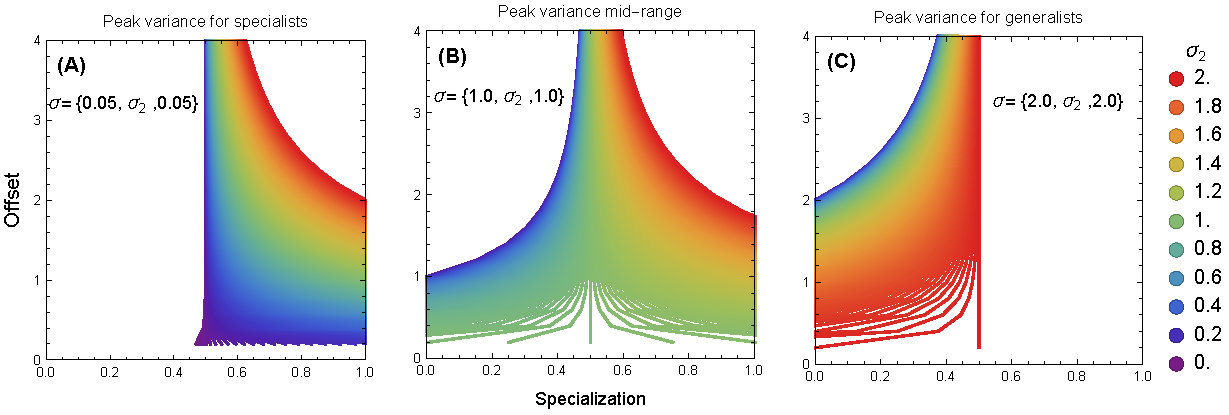
\includegraphics[width=1\textwidth]{fig_specvar.pdf}
\caption{
}
\end{figure}



\begin{figure}[h!]
\centering
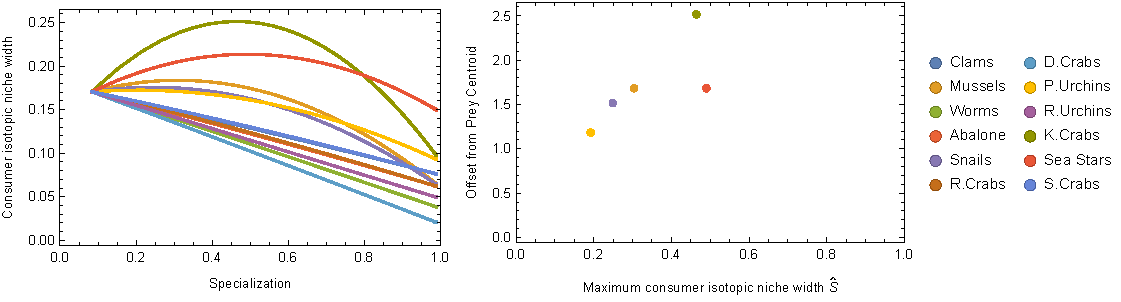
\includegraphics[width=1\textwidth]{fig_ottervar.pdf}
\caption{
}
\end{figure}


\end{document}
